%TODO: Look for CPD / activity detection research in literature. (Choudhury?)

\section{Top-Down Approach}
\label{sec:topdown}

\subsection{Change-Point Detection}
For this approach, the data was split into non-overlapping segments for
featurization using techniques from the statistical field of change-point
detection. Change-point detection has found application in many problem domains
that require analysis of time series data from dynamic systems, including
failure detection \cite{bae13}, quick detection of attacks on computer networks
\cite{tartakovsky06}, and monitoring of heartbeat fluctuations during
sleep \cite{staudacher05}. Change-point detection techniques assume that each
tick of a time series is a draw from some probability
distribution, but that the distribution may suddenly change as time passes.
The goal is to predict when these changes have occurred.
A \emph{score} is generated for each time tick, and if the score is
above a given threshold a change is predicted to have occurred between that tick
and its immediate predecessor. To generate a score at a time tick, a window of
data that immediately preceeds it (the \emph{reference data}) is compared to it
along with a window of data that immediately follows it (the \emph{test data}), 
as shown in Figure \ref{fig:cpd_ref_test}.

\begin{figure}
 \centering
 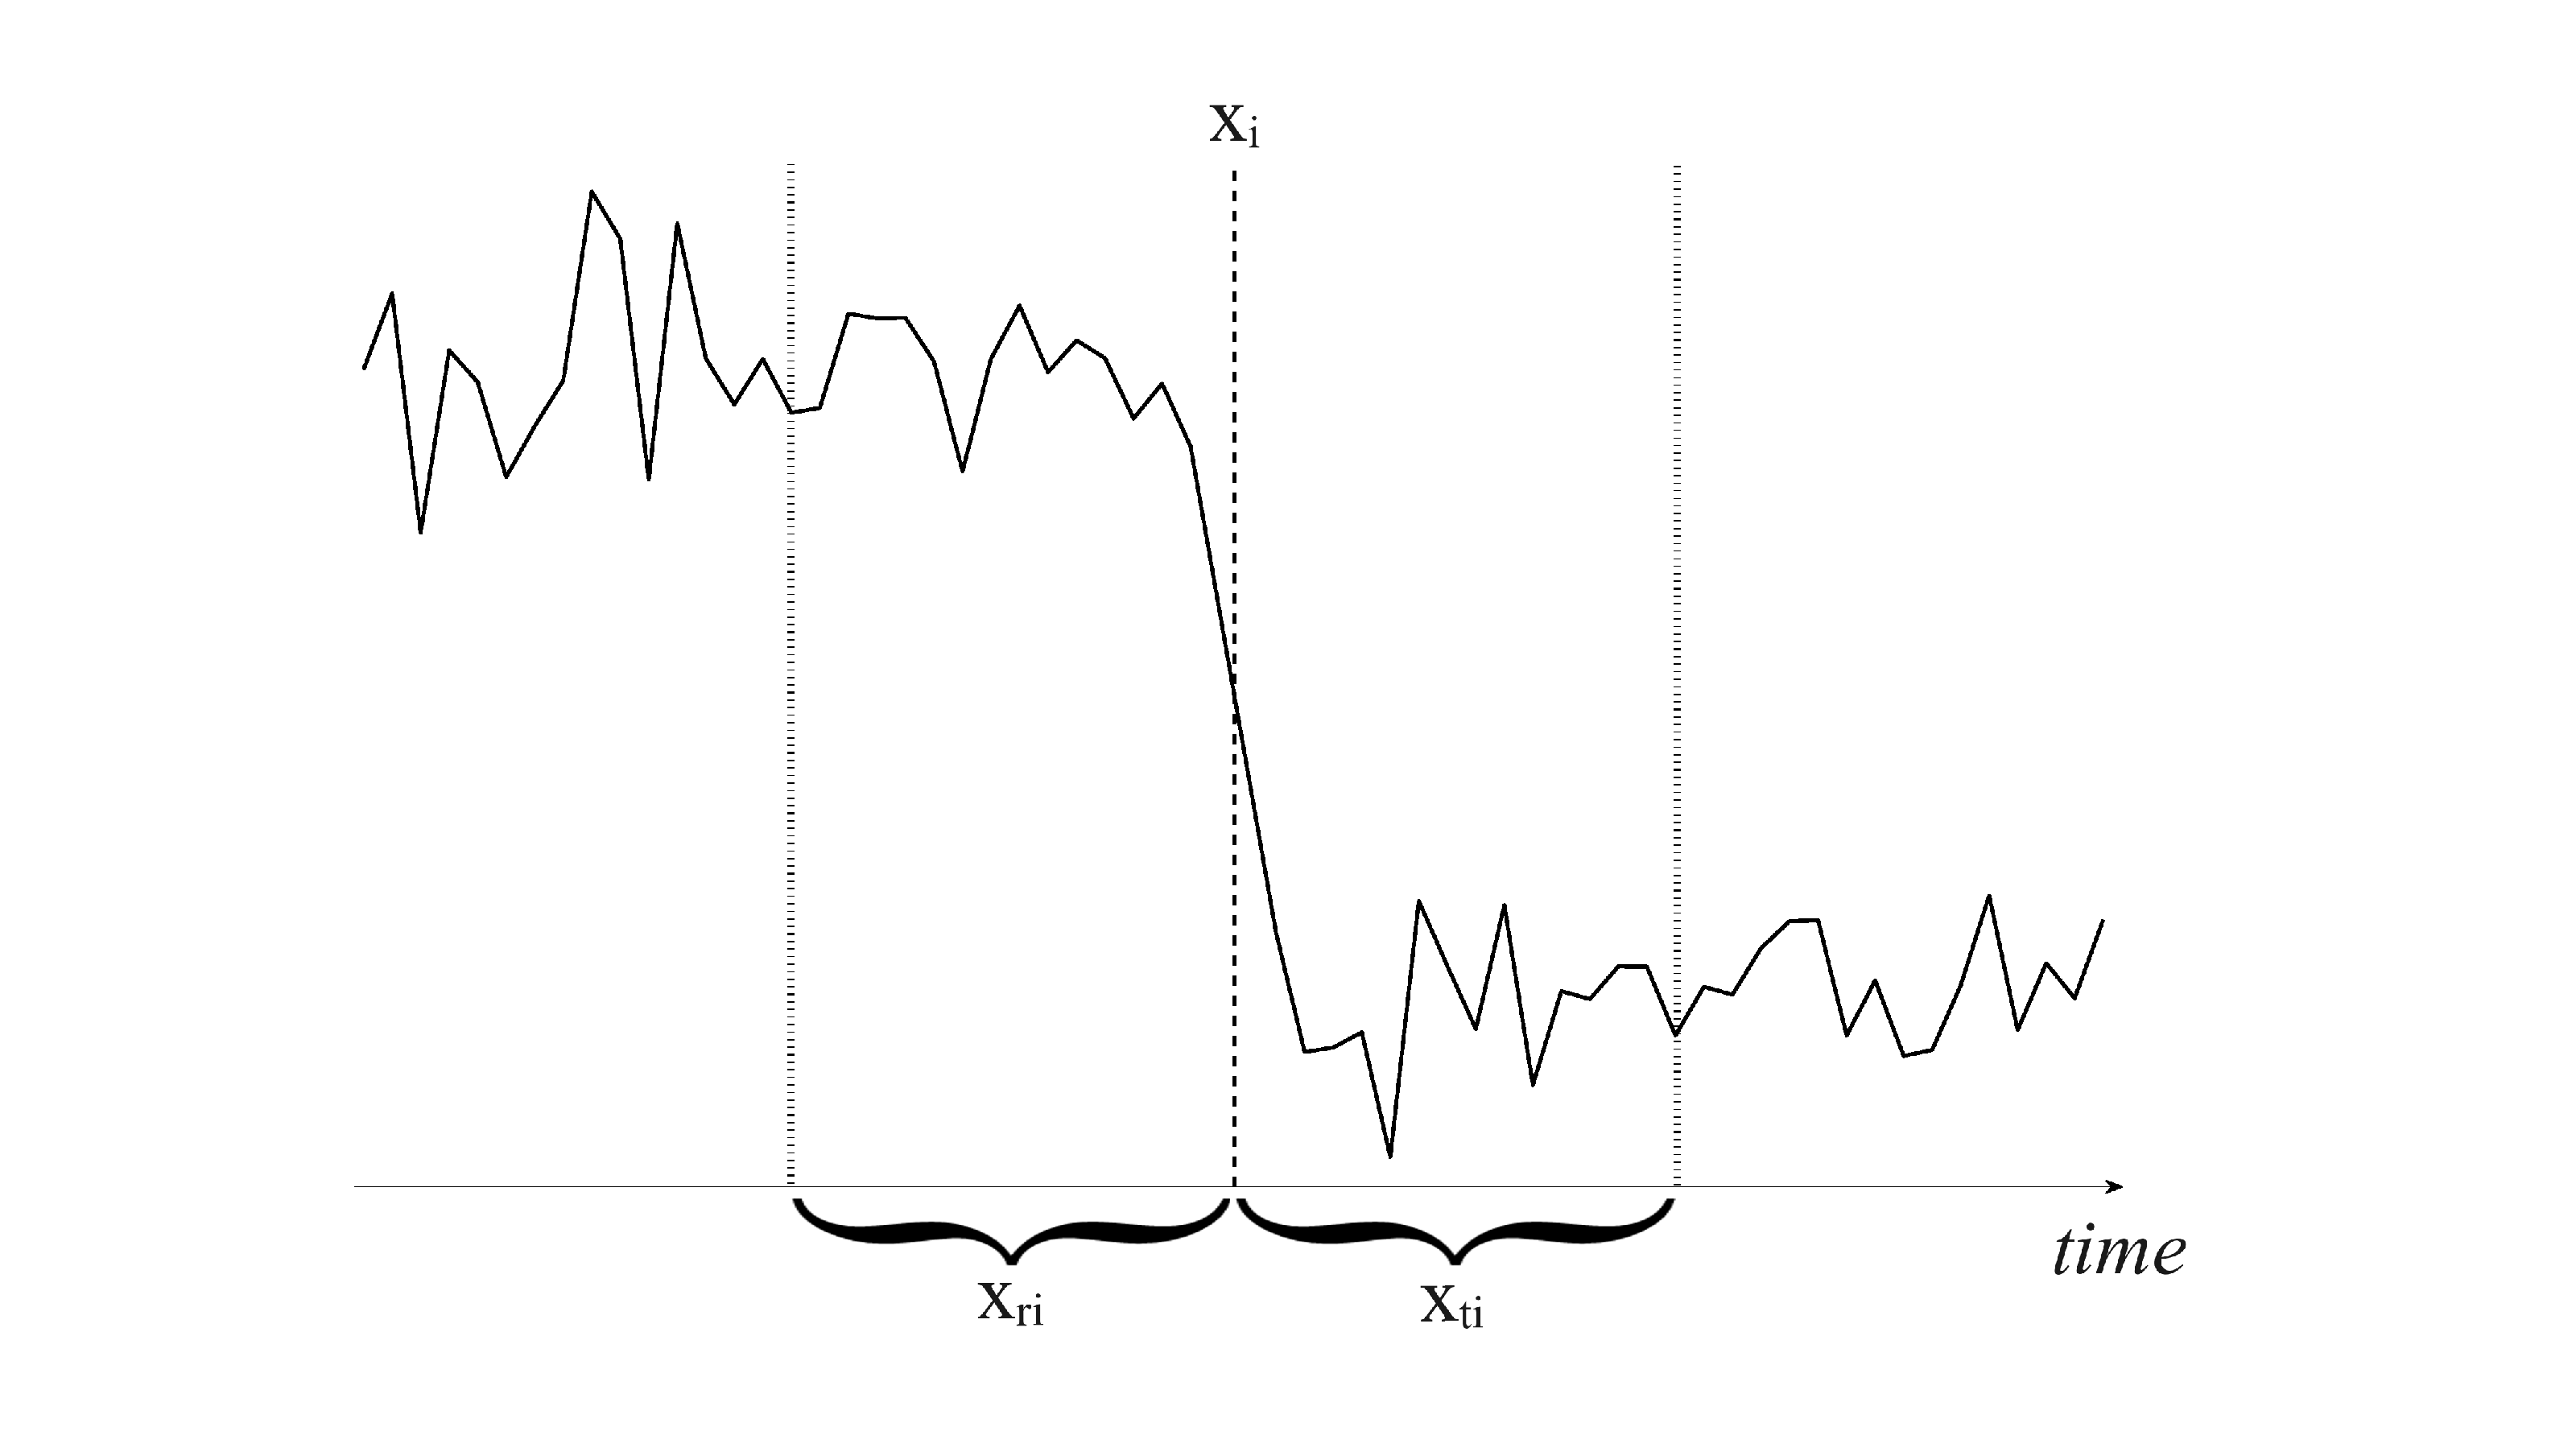
\includegraphics[scale=0.25]{cpd_ref_test.pdf}
 \caption{Reference and Test Data}
 \label{fig:cpd_ref_test}
\end{figure}

Model-based approaches to change-point detection assume that each tick in
a time series is a draw from some underlying probability distribution.
Scores are generated by estimating the distribution of the reference data
and the test data, and then by calculating the likelihood
that the two distributions are different. Parametric estimation methods have
been employed where is it reasonable to assume that the given data belongs to a
particular family of distributions \cite{thatte11}. Non-parametric methods have
also been found to be viable where no such modeling
assumptions are reasonable \cite{matteson12}. Distance-based approaches such as
Singular Spectrum Analysis generate scores through other metrics of 
dissimilarity or difference between the reference data and the test data
\cite{moskvina03}.
Notationally, we say that for each tick $i$ in a time series:

\[
s(i) = D(X_r(i), X_t(i))
\]

Where $s(i)$ is the score of the $i$th tick, $X_r(i)$ is the reference
data associated with the $i$th tick, $X_t(i)$ is the test data
associated with the $i$th tick, and $D(A,B)$ is a function that computes the
dissimiliarity between a matrix of data $A$ and matrix of data $B$. $D(A,B)$
varies between change-point algorithms. Note that for a given
algorithm it may not be possible to generate scores right at the very beginning
of the time series (insufficient reference data) or at the very end of a time
series (insufficient test data).

\subsection{Experimental Setup}

Each dataset that we tested consisted of multiple time series gathered from
a number of different subjects. To perform an experiment on a dataset we
began by partitioning the set of time series into disjoint subsets of training,
validation, and testing data. Each individual time series was then partitioned
into a set of non-overlapping windows, and each window was converted into its
own feature vector. Once the dataset was featurized, the experiment could be
treated as a typical classification problem. Classifiers were built with the
training set, and tuned (when necessary) on the validation set. 
Finally, the tuned model was evaluated by prediction on the testing set.
A visualization of the data lifecycle is shown in Figure
\ref{fig:cpd_lifecycle}.
 
\begin{figure}
 \centering
 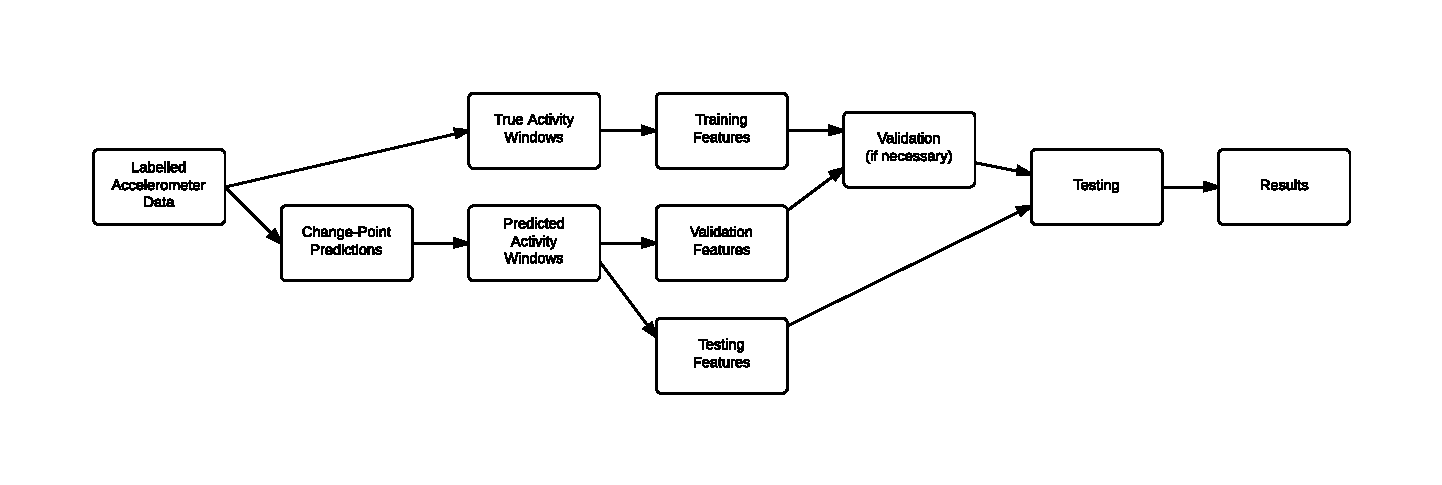
\includegraphics[scale=0.15]{cpd_lifecycle.pdf}
 \caption{Data Lifecycle of Change-Point Detection Experiments}
 \label{fig:cpd_lifecycle}
\end{figure}

There are many different modeling assumptions and associated algorithms
for generating change-point detection scores, and one simple baseline approach
that we wanted to test was the Shewhart Control Chart \cite{shewhart26}.
This approach assumes that the reference data is drawn from a multivariate
normal distribution, and that scores are calculated by the Mahalanobis distance
of the target time tick from the estimated multivariate normal:

\[
s(i) = \sqrt{[\bar{X}_r(i) - X(i)]_T \; \frac{1}{S_r(i)} \; [\bar{X}_r(i) - X(i)]}
\]

where $\bar{X}_r(i)$ is the sample mean of the reference data, $S_r(i)$
is the sample covariance matrix of the reference data, and $X(i)=X_t(i)$ is
the $i$th data point.

We were also interested in testing the performance of a newer and more
sophisticated change-point detection algorithm: the
Kullback-Leibler Importance Estimation Procedure (KLIEP),
introduced by Kawahara and Sugiyama \cite{sugiyama09} \cite{sugiyama08}.
This approach generates scores using the Kullback-Leibler (KL)
divergence between the reference data and the test data. One method of doing this
is to estimate the density of the reference distribution and test distribution
separately, and then compare them using a likelihood ratio
(known in the change-point detection literature as \emph{importance}). 
Instead, KLIEP estimates the importance directly using a non-parametric model.

Let the estimate of the importance $\hat{R}$ be represented by this model:

\[
\hat{R} = \frac{p_t}{\hat{p}_r} = \sum_{i=1}^{T_t} \alpha_j K_G(X_{rt},X_t(j))
\]

Where $p_r$ and is the probability density of the reference data,
$p_t$ is the probability density of the test
data, $T_t$ is the number of ticks in the test window, $\alpha$ is a
vector of model parameters to solve for, $X_{rt}$ is the concatenation of the reference and the
test data, $X_t(i)$ is the $i$th element of the test data,
and $K_G[A,B]$ is the Gaussian kernel with width $\sigma$:

\[
K_G[A,B] = \exp \left(-\frac{||A-B||^2}{2\sigma^2}\right)
\]

Now solve for $\alpha$ so that the empirical KL divergence between $\hat{p}_t$ and
$p_t = \hat{R}p_r$ is minimized, which is equivalent to the following convex optimization
problem:

\[
\begin{dcases}
 \max_{\alpha} \quad \sum_{j=1}^{T_t} \, \log \left( \sum_{k=1}^{T_t} \alpha_k K_G[X_t(j), X_t(k)] \right) \\
 \,\, \text{s.t.} \quad\, \frac{1}{T_r} \sum_{j=1}^{T_r} \sum_{k=1}^{T_t} \alpha_k K_G[X_r(j),X_t(k)] = 1 \\
 \qquad \quad \text{and} \; \alpha_1 \ldots \alpha_{T_t} \ge 1
\end{dcases}
\]

Finally, the scores that we wish to generate are just the estimate of the importance given by the
solution to the complex optimization problem, i.e. $s(i) = \hat{R}(i)$.

Since this approach uses a Gaussian kernel, it requires the selection of
a kernel width $\sigma$ for each time tick. We used an implementation of
KLIEP that is available at Sugiyama's website, which included a cross-validation
procedure for the value of $\sigma$. The CV procedure chooses a number of disjoint
splits of the test data along with a number of different candidate $\sigma$'s, and runs
KLIEP with each combination of split and candidate $\sigma$. Then it chooses the candidate $\sigma$
that, on the average across all of the splits, maximizes the KL divergence (the
$\max_{\alpha}$ equation above) the most.

For the OSU Hip dataset, we used this CV procedure to choose the kernel width.
This computationally intensive approach was
impractical for the UQ dataset because it is orders of magnitude larger,
so instead of running it on every tick of that data, we ran the CV procedure on
a small sample of data. From this smaller sample we were able
to empirically identify 0.01 as a plausible $\sigma$, and so fixed $\sigma$
at that value for our experiments on that dataset.

Our selection of reference and test window sizes were informed by two considerations:
first that the window sizes contain enough data to accurately model the
reference and test distributions, and second that the window sizes were small enough
to detect activity changes at real time speeds.
Previous research \cite{zheng12} found that a reference window size of 10
seconds contained just enough information to discriminate well between OSU Hip activities.
Since this window size worked well in previous experiments, and since the 
activities of the UQ dataset were comparable in average length, we decided to
fix our reference window size at 10 seconds for both datasets. Because we were interested in
minimizing detection time, and because 1 second was the smallest window that
we felt could provide some information about an activity, we fixed our test
window size at 1 second for both datasets.

Once change-point detection scores were generated, we tested a number of threshold values that determined which
scores were high enough to be considered a predicted change-point.
Threshold values were chosen by considering the false positive rates of
change prediction for the change-point detection algorithms. A smaller false positive rate
corresponded to a higher and more conservative threshold, which split the
time series into fewer segments. A larger false positive rate
corresponded to a lower threshold, which split the time series into more segments.
